\documentclass[output=paper]{langscibook} 
\ChapterDOI{10.5281/zenodo.5082464}

\author{Marcin Wągiel\affiliation{Masaryk University}}

\title{Slavic derived collective nouns as spatial and social clusters}
\abstract{In this chapter, I examine two types of Slavic derived collective nouns, namely spatial collectives such as Polish \textit{kwiecie} `clump of flowers' and social collectives like \textit{duchowieństwo} `collective of priests, clergy'. While the former refer to collections of objects perceived as coherent spatial configurations, the latter denote groups of human individuals performing a salient social role. Building on \citet{grimm2012number} and \citet{zobel2017sensitivity}, I propose an analysis that treats the Slavic derived collective nouns in question as predicates true of spatial and social clusters, respectively. The proposal extends mereotopology to the abstract domain of social roles. 

\keywords{collective nouns, social nouns, mereotopology, roles}}

\begin{document}
\SetupAffiliations{mark style=none}
\maketitle

\section{Introduction}\label{wan:sec:introduction}

A puzzling property of collective nouns is that they simultaneously evoke a sense of plurality and singularity (\citealt[195]{jespersen1924philosophy}, \citealt{gil1996maltese}). For instance, a team is constituted by a number of players but at the same time it seems to be something more than just a collection of players. It is an entity in itself with an internal structure, independent goals and an elaborate way of functioning. As such it seems to be a unit of a higher type. Though it is commonly assumed that collectives are specific to the domain of individuals, see widely discussed examples like \REF{wan:ex:collectives-individuals}, in fact the category is much more general and can be identified also in the domain of eventualities, as in \REF{wan:ex:collectives-eventualities}, as well as abstract objects such as numbers, see \REF{wan:ex:collectives-numbers}.

\ea \ea committee of women, deck of cards\label{wan:ex:collectives-individuals}
\ex series of unfortunate events, sequence of murders\label{wan:ex:collectives-eventualities}
\ex sequence of integers, set of real numbers\label{wan:ex:collectives-numbers}
\z
\z

\noindent For a long time, it was standardly taken for granted that collective nouns constitute a uniform category (e.g., \citealt{landman1989groupsi,barker1992group,schwarzschild1996pluralities}). However, recent findings suggest that there are different kinds of such expressions (\citealt{joosten2010collective,pearson2011new,de_vries2015shifting,henderson2017swarms,zwarts2020contiguity}; for a recent overview, see \citealt{de_vries-toappear-collective}). In this paper, I will argue that Slavic derivational morphology reflects two modes of collectivity. In particular, I will examine two types of derived collectives in Slavic exemplified by the Polish nouns in \REF{wan:ex:polish-collectives}.\footnote{The orthographic differences between the singular and collective forms in \REF{wan:ex:polish-collectives}, specifically \textit{a}~:~\textit{e}, \textit{t}~:~\textit{ci}, $\varnothing$~:~\textit{ie} and \textit{n}~:~\textit{ń} all represent standard morphonological alternations in Polish. Notice also that the two classes in \REF{wan:ex:polish-collectives} are uncountable aggregate nouns while most of the literature focuses mainly on countable collectives \citep[but see][]{de_vries-toappear-collective}.}

\ea \label{wan:ex:polish-collectives} \ea {\gll kwiat $\Rightarrow$ kwieci-e\\
    flower { } {flower-\textsc{coll}}\\ %\hfill (Polish)
    \glt `flower' \hspace{0.2cm} `clump(s) of flowers'
    }\label{wan:ex:polish-kwiecie}
\ex {\gll duchowny $\Rightarrow$ duchowień-stwo\\
priest { } {priest-\textsc{coll}}\\
\glt `priest' \hspace{0.95cm} `collective of priests, clergy' \hfill (Polish)
}\label{wan:ex:polish-duchowienstwo}
\z
\z

\noindent The main claim of this paper is that both types of Slavic derived collective nouns designate clusters, i.e., structured configurations of objects. I will argue that \textsc{spatial} collectives like that in \REF{wan:ex:polish-kwiecie} denote spatial clusters, i.e., topological arrangements of entities in physical space, whereas \textsc{social} collectives as in \REF{wan:ex:polish-duchowienstwo} refer to social clusters, i.e., abstract configurations of roles individuals can bear in social space. 

The paper is outlined as follows. In \sectref{wan:sec:modes-of-collectivity}, I discuss different ways in which collective inferences can arise. \sectref{wan:sec:types-of-collectives} revises different types of collectives analyzed in the literature, specifically those that construe a group in terms of a topological configuration of their constituents as opposed to those that encode an abstract notion of a group independent of the spatial arrangement of its members. In \sectref{wan:sec:slavic-derived-collectives}, I explore derived spatial and social collectives across Slavic languages with a special focus on Polish. In \sectref{wan:sec:mereotopology} and \sectref{wan:sec:roles}, I introduce a theoretical framework including mereotopology and an extension of the ontology with roles. In \sectref{wan:sec:collectives-as-clusters}, I propose an extended mereotopological approach on which both spatial and social collectives are analyzed as clusters. Finally, \sectref{wan:sec:conclusion} concludes the paper.

\section{Modes of collectivity}\label{wan:sec:modes-of-collectivity}

According to \citeauthor{landman1989groupsi} (\citeyear{landman1989groupsi,landman2000events}), collective inferences arise due to the special nature of the argument of the predicate, i.e., the fact that it denotes a group rather than an individual. According to this account, there are three ways in which one can construe a collective interpretation \citep[165--169]{landman2000events}. Specifically, a group can be obtained via (i)~collective body formation, (ii)~collective action and (iii)~collective responsibility, as illustrated by the corresponding examples in \REF{wan:ex:modes}.

\ea\label{wan:ex:modes} \ea The boys touch the ceiling.\label{wan:ex:modes-body}
\ex The boys carried the piano upstairs.\label{wan:ex:modes-action}
\ex The gangsters killed their rivals. \hfill \citep[165--167]{landman2000events}\label{wan:ex:modes-responsibility}
\z
\z

\noindent The first mechanism creates a group via so-called collective body formation. \figref{wan:fig:body-distributive} depicts the distributive reading of \REF{wan:ex:modes-body}. Here, each boy touches the ceiling himself. What is more interesting for our purposes though is the collective reading illustrated by the scenario in \figref{wan:fig:body-collective}. Although not every boy touches the ceiling himself, the sentence is true because the boys have put themselves in a particular spatial configuration, i.e., a pyramid, in order to touch the ceiling together. Such a collective body constitutes an independent object in its own right. 

\begin{figure}[h]
\RawFloats
\centering
\begin{minipage}[b]{0.5\textwidth}
\centering
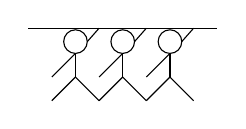
\begin{tikzpicture}
\draw (-0.1,0.02) -- (2.3,0.02);
  \draw (0.5,-0.15) circle (0.15cm);
  \draw (0.5,-0.3) -- (0.5,-0.6);
        \draw (0.2,-0.6) -- (0.5,-0.3);
        \draw (0.65,-0.15) -- (0.8,0.02);
        \draw (0.5,-0.6) -- (0.8,-0.9);
        \draw (0.5,-0.6) -- (0.2,-0.9);
  \draw (1.1,-0.15) circle (0.15cm);
  \draw (1.1,-0.3) -- (1.1,-0.6);
        \draw (0.8,-0.6) -- (1.1,-0.3);
        \draw (1.25,-0.15) -- (1.4,0.02);
        \draw (1.1,-0.6) -- (1.4,-0.9);
        \draw (1.1,-0.6) -- (0.8,-0.9);
  \draw (1.7,-0.15) circle (0.15cm);
  \draw (1.7,-0.3) -- (1.7,-0.6);
        \draw (1.4,-0.6) -- (1.7,-0.3);
        \draw (1.85,-0.15) -- (2.0,0.02);
        \draw (1.7,-0.6) -- (2.0,-0.9);
        \draw (1.7,-0.6) -- (1.4,-0.9);
\end{tikzpicture}
\caption{Distributive reading of \REF{wan:ex:modes-body}}
\label{wan:fig:body-distributive}
\end{minipage}%
\begin{minipage}[b]{0.5\textwidth}
\centering
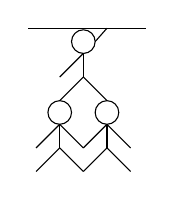
\begin{tikzpicture}
\draw (-0.2,0.02) -- (1.3,0.02);
  \draw (0.5,-0.15) circle (0.15cm);
  \draw (0.5,-0.3) -- (0.5,-0.6);
        \draw (0.2,-0.6) -- (0.5,-0.3);
        \draw (0.65,-0.15) -- (0.8,0.02);
        \draw (0.5,-0.6) -- (0.8,-0.9);
        \draw (0.5,-0.6) -- (0.2,-0.9);
  \draw (0.2,-1.05) circle (0.15cm);
  \draw (0.2,-1.2) -- (0.2,-1.5);
        \draw (-0.1,-1.5) -- (0.2,-1.2);
        \draw (0.5,-1.5) -- (0.2,-1.2);
        \draw (-0.1,-1.8) -- (0.2,-1.5);
        \draw (0.5,-1.8) -- (0.2,-1.5);
  \draw (0.8,-1.05) circle (0.15cm);
  \draw (0.8,-1.2) -- (0.8,-1.5);
        \draw (0.5,-1.5) -- (0.8,-1.2);
        \draw (1.1,-1.5) -- (0.8,-1.2);
        \draw (0.5,-1.8) -- (0.8,-1.5);
        \draw (1.1,-1.8) -- (0.8,-1.5);
\end{tikzpicture}
\caption{Collective reading of \REF{wan:ex:modes-body}}
\label{wan:fig:body-collective}
\end{minipage}
\end{figure}

On the other hand, the collective interpretation of \REF{wan:ex:modes-action} results from the fact that the constituent individuals, i.e., the boys, performed a collective action, i.e., carried the piano upstairs together. For an activity to be perceived as such it typically needs to involve a shared goal and simultaneous movement. Individuals involved in collective action often occupy determined positions with respect to each other and move along parallel paths. All those features have the result that a plurality is likely to be perceived as one unit. 

Finally, the collective interpretation of \REF{wan:ex:modes-responsibility} does not arise as a result of a particular spatial configuration of the individuals involved in an event but rather in a more abstract way. The sentence would be true even in a scenario when only one gangster actually pulled the trigger since what is crucial here is shared commitments and collective responsibility stemming from the members' involvement in a particular type of social organization.

Though \citeauthor{landman2000events}'s distinctions are very useful and instructive, it seems that the cases discussed above generally reduce to the two mechanisms of group formation intuitively characterized in \figref{wan:fig:modes-of-collectivity} \citep{zwarts2020contiguity}. The left-hand part of \figref{wan:fig:modes-of-collectivity} represents a process in which the individuals are recognized as making up a higher order unit due to their spatial configuration. As a result of topological contiguity and relative proximity, a perception of a whole that is more than a mere sum of the parts arises. By contrast, the right-hand part of \figref{wan:fig:modes-of-collectivity} represents a reverse process in which collectivity is regarded as basic. As such it is conceptualized irrespective of the spatial configuration of the members of the group. Instead, it is taken as some abstract connection holding between them, e.g., a web of social relations. For the purpose of this paper, I will refer to the mechanisms in \figref{wan:fig:modes-of-collectivity} as the two \textsc{modes of collectivity}. Specifically, I will call them the \textsc{spatial mode} and the \textsc{social mode}, respectively.

\begin{figure}[h!]
\centering
\begin{tikzpicture}
  \draw (-0.2,0.0) circle (0.2cm);
  \draw (0.5,0.45) circle (0.2cm);
  \draw (-0.75,0.5) circle (0.2cm);
  \draw (-1.1,-0.2) circle (0.2cm);
  \draw (-0.5,-0.5) circle (0.2cm);
  \draw (0.6,-0.6) circle (0.2cm);
  \draw (1.0,0.2) circle (0.2cm);
  \node[draw, single arrow,
        minimum height=7mm, minimum width=5mm,
        single arrow head extend=2mm,
        anchor=west] at (1.65,0.0) {};
  \node[draw, single arrow,
        minimum height=7mm, minimum width=5mm,
        single arrow head extend=2mm,
        anchor=west, rotate=-180] at (6.35,0.0) {};
  \draw (4.0,0.0) ellipse (1.5cm and 1.0cm);
  \draw (3.8,0.0) circle (0.2cm);
  \draw (4.5,0.45) circle (0.2cm);
  \draw (3.25,0.5) circle (0.2cm);
  \draw (2.9,-0.2) circle (0.2cm);
  \draw (3.5,-0.5) circle (0.2cm);
  \draw (4.6,-0.6) circle (0.2cm);
  \draw (5.0,0.2) circle (0.2cm);
  \draw (8.0,0.0) ellipse (1.5cm and 1.0cm); 
\end{tikzpicture}
\caption{Modes of collectivity}
\label{wan:fig:modes-of-collectivity}
\end{figure}

While \citeauthor{landman2000events}'s collective body formation, recall \REF{wan:ex:modes-body}, is a clear case of the spatial mode, collective responsibility, recall \REF{wan:ex:modes-responsibility}, certainly involves being part of some social entity independent of the position of its members. On the other hand, the cases of collective action exemplified in \REF{wan:ex:modes-action} can relate to either the spatial or the social mode of collectivity, depending on a particular situation.\footnote{Though \REF{wan:ex:modes-action} seems to neatly fit the spatial mode of collectivity, one can easily imagine actions that require the coordination of multiple activities performed at different times and locations: 

\ea The personnel launched the space shuttle.\label{wan:ex:shuttle}
\z}

\section{Types of collectives}\label{wan:sec:types-of-collectives}

Differentiating between two independent modes of collectivity is an important insight not only from the perspective of general conceptual considerations. It turns out that natural language appears to be sensitive to the different ways a group can be construed. In particular, there is a growing body of evidence demonstrating that in fact there are (at least) two types of collective nouns, namely (i)~\textsc{social collectives} designating organizations constituted by their members, e.g., \textit{committee (of women)}, \textit{team (of players)} and \textit{gang (of counterfeits)}, and (ii)~\textsc{spatial collectives} referring to topological configurations of objects, e.g., \textit{bunch (of flowers)}, \textit{pile (of dishes)} and \textit{crowd (of people)} \citep{pearson2011new,de_vries2015shifting,henderson2017swarms,zwarts2020contiguity}.\footnote{Notice that different terms have been used to describe the distinction, e.g., \citeauthor{pearson2011new} differentiates between committee and collection nouns, \citeauthor{henderson2017swarms} distinguishes between group and swarm nouns, whereas \citeauthor{zwarts2020contiguity} talks about club and crowd nouns. However, since the expressions designated by these labels encode also (in)animacy (see below), I will use the more general terms social and spatial collectives instead.}

A number of diagnostics to distinguish the two types of collective nouns have been proposed in the literature, e.g, (i)~plural agreement in British and Canadian English, (ii)~ability to antecede plural pronouns, (iii)~embedding in partitive constructions, (iv)~quantificational domain of \textit{half}, (v)~reference to larger cardinalities, (vi)~truth conditions of negated existential statements, (vii)~compatibility with spatial modifiers and (viii)~compatibility with certain expressions such as the Dutch noun \textit{lid} `member'. Nevertheless, only (v--viii) turn out to be reliable diagnostics. In order to show that, let us look more closely at each of them.\footnote{I would like to thank Kurt Erbach and Peter Sutton for their judgments concerning American and British English, respectively, as well as for the discussion of the data to be reported below.}

\subsection{Flawed diagnostics}\label{wan:sec:flawed-diagnostics}

It has been observed that in British and Canadian English nouns such as \textit{committee} allow for plural agreement \citep{barker1992group}, whereas expressions like \textit{bunch of flowers} do not \citep{pearson2011new}, as demonstrated in \REF{wan:ex:agreement}. At first blush, the contrast seems to stem from the spatial/social distinction.

	\ea\label{wan:ex:agreement}
		\ea[]{The committee are old. \hfill \citep[89]{barker1992group}}\label{wan:ex:agreement-commitee}
		\ex[*]{The bunch of flowers are tall. \hfill \citep[163]{pearson2011new}}\label{wan:ex:agreement-bunch}
    \z
    \z

\noindent However, this test ignores the role animacy plays in the behavior of collective nouns \citep[see][Ch.~6]{de_vries2015shifting} and it turns out that the agreement pattern in \REF{wan:ex:agreement-commitee} is sensitive to the distinction between animate and inanimate collections rather than that between social and spatial collections. To demonstrate this, let us consider a noun like \textit{crowd}, which designates a spatial configuration and yet can trigger plural agreement on the verb in British English, as in \REF{wan:ex:agreement-crowd}. That is because \textit{crowd} refers to a collection of animate individuals.

	\ea[]{The crowd are cheerful.}\label{wan:ex:agreement-crowd}
    \z

\noindent According to the second diagnostic \citep[proposed by][]{henderson2017swarms}, only social collectives can be used as an antecedent of the plural pronoun \textit{they}, see \REF{wan:ex:anaphora-committee}. On the other hand, spatial collectives allow only for singular anaphora, as witnessed by the infelicity of the second sentence in \REF{wan:ex:anaphora-bouquet}.

	\ea\label{wan:ex:anaphora}
		\ea[]{The committee is in the backyard. They are by the river.}\label{wan:ex:anaphora-committee}
		\ex[]{The bouquet is in the backyard. \#They are by the river. \\ \hfill \citep[170]{henderson2017swarms}}\label{wan:ex:anaphora-bouquet}
    \z
    \z

\noindent However, after neutralizing the confounding factor of animacy, we can see in \REF{wan:ex:anaphora-crowd} that animate spatial collectives pattern with social collectives such as \REF{wan:ex:anaphora-committee}.\footnote{In fact, \citeauthor{henderson2017swarms} himself acknowledges that the nouns \textit{swarm} and \textit{horde} unexpectedly enable plural anaphora.}

	\ea[]{The crowd is in the backyard. They are by the river.}\label{wan:ex:anaphora-crowd}
	\z

\noindent Another alleged diagnostic concerns the behavior of collective nouns in partitives. \citet{pearson2011new} reports that social collectives such as \textit{committee} can be embedded in partitive constructions headed by a count determiner, as in \REF{wan:ex:partitive-committee}, whereas spatial collective nominals like \textit{bunch of flowers} cannot, see \REF{wan:ex:partitive-bunch}. 

	\ea\label{wan:ex:partitive} 
		\ea[]{Three of the committee came to the meeting.}\label{wan:ex:partitive-committee}
		\ex[*]{Three of the bunch of flowers had died. \hfill \citep[162--163]{pearson2011new}}\label{wan:ex:partitive-bunch}
    \z	
    \z

\noindent But again, the contrast in \REF{wan:ex:partitive} does not reflect the spatial/social distinction, but rather it is due to animacy. As evidenced by the grammaticality of \REF{wan:ex:partitive-crowd}, the animate spatial collective \textit{crowd} displays the same behavior as the social collective in \REF{wan:ex:partitive-committee}.

\ea[]{Three of the crowd were killed and several wounded.}\label{wan:ex:partitive-crowd}
\z

\noindent Finally, \citeauthor{pearson2011new} observes that while \REF{wan:ex:denotation-bunch} and \REF{wan:ex:denotation-wall} can quantify over any part of the wall and the bouquet (and not only individual flowers and bricks), respectively, \REF{wan:ex:denotation-committee} quantifies exclusively over individual committee members. Therefore, she postulates that social and spatial collectives differ semantically in that the former have a plural denotation, while the latter have an atomic denotation. 
	
	\ea\label{wan:ex:denotation} 
		\ea[]{Half of the committee had been painted yellow.}\label{wan:ex:denotation-committee}
		\ex[]{Half of the bunch of flowers had been painted yellow.}\label{wan:ex:denotation-bunch}
		\ex[]{Half of the wall had been painted yellow.\label{wan:ex:denotation-wall} \hfill \citep[161--163]{pearson2011new}}
    \z	
    \z

\noindent However, as already pointed out by \citet{zwarts2020contiguity}, this test also neglects the effect of animacy. In examples with animate social collectives such as \REF{wan:ex:denotation-crowd}, what is quantified over are individual persons making up the crowd rather than arbitrary material parts of the crowd such as people's limbs. Thus, \REF{wan:ex:denotation-crowd} patterns with \REF{wan:ex:denotation-committee} despite the fact that \textit{crowd} is not a social collective noun. 

	\ea[]{Half of the crowd had been painted yellow. \hfill \citep[551]{zwarts2020contiguity}}\label{wan:ex:denotation-crowd}
	\z

\noindent I conclude that the four tests discussed above fail as reliable diagnostics for distinguishing between social and spatial collective nouns. Instead, what they show is that animate and inanimate collectives behave differently. Let us now examine the remaining four tests, which as I will argue do a better job at discerning the spatial/social distinction.

\subsection{More reliable diagnostics}\label{wan:sec:more-reliable-diagnostics}

\noindent As recognized by \citet{henderson2017swarms}, referents of spatial collectives must be constituted by a sufficiently large number of entities. On the other hand, referents of social collective nouns need not, as witnessed by the contrast in \REF{wan:ex:plurality}.
	
	\ea\judgewidth{\#}\label{wan:ex:plurality} 
		\ea[]{Bill needs to learn to cook for a family of two.}\label{wan:ex:plurality-family} 
		\ex[\#]{John planted a grove of two redbud trees. \hfill \citep[167]{henderson2017swarms}}\label{wan:ex:plurality-grove}
    \z	
    \z

\noindent In the previous section, we have discussed the class of animate spatial collectives such as \textit{crowd (of people)}. An interesting question arises whether there is evidence for an inverse category designating inanimate social collections. Though at first blush such entities may seem impossible, notice that the development of information technology and logistics gives rise to higher order configurations of inanimate objects, which are based on function rather than spatial proximity. Hence, I posit that expressions such as \textit{fleet (of trucks)} and \textit{network (of computers)} are good candidates for inanimate social collectives and the comparison between \REF{wan:ex:plurality-fleet} and \REF{wan:ex:plurality-family} shows that in fact they pattern with their animate counterparts.

	\ea[]{The company owns a fleet of two trucks for unexpected deliveries.}\label{wan:ex:plurality-fleet}
    \z

\noindent Another important observation by \citeauthor{henderson2017swarms} is that individuals designated by spatial collectives must occupy the same region of space. Consider, for instance, the spatial entailments in \REF{wan:ex:entailment-committee} and \REF{wan:ex:entailment-bouquet}. While social collectives are insensitive to the locations of their constituent members, spatial collections may cease to exist if the topological configuration of the entities that make them up is rearranged.
	
	\ea\judgewidth{$\nvDash$}\label{wan:ex:entailment-committee} 
		\ea[]{Each member of the committee travels to a different state to visit family.}\label{wan:ex:entailment-committee1} 
		\ex[$\nvDash$]{The committee no longer exists. \hfill \citep[168]{henderson2017swarms}}\label{wan:ex:entailment-committee2} 
	\z	
	\ex\judgewidth{$\vDash$}\label{wan:ex:entailment-bouquet}		
		\ea[]{Someone takes each flower from the bouquet and places it in a different room of the house.}\label{wan:ex:entailment-bouquet1} 
		\ex[$\vDash$]{The bouquet no longer exists. \hfill \citep[168]{henderson2017swarms}}\label{wan:ex:entailment-bouquet2}
    \z	
    \z

\noindent The behavior of inanimate social collectives like the one in \REF{wan:ex:entailment-fleet}, which is on a par with \REF{wan:ex:entailment-committee} and contrasts with \REF{wan:ex:entailment-bouquet}, corroborates the validity of the test based on truth conditions of negated existential statements.

	\ea\judgewidth{$\nvDash$}\label{wan:ex:entailment-fleet}
	\ea[]{Each truck from the fleet travels to a different state to deliver goods.}\label{wan:ex:entailment-fleet1}
	\ex[$\nvDash$]{The fleet no longer exists.}\label{wan:ex:entailment-fleet2}
    \z
    \z

\noindent The remaining two diagnostics are based on Dutch data examined by \citet{zwarts2020contiguity}, who provides a number of linguistic contrasts between social and spatial collectives. First, let us consider certain constraints on spatial modification. For instance, the Dutch preposition \textit{midden in} `in the middle' specifies precisely a spatial location. The contrast in \REF{wan:ex:spatial} shows that it is felicitous with spatial collectives since they demarcate a topological region, whereas it is strange with social collectives, which lack this property.	
	
	\ea\label{wan:ex:spatial} 
		\ea[?]{\gll midden in een comité\\
		middle in a committee\\
		\glt Intended: `in the middle of a committee'\label{wan:ex:spatial-committee}}
		\ex[]{\gll midden in een menigte\\
		middle in a crowd\\
		\glt `in the middle of a crowd' \hfill \citep[Dutch;][547]{zwarts2020contiguity}\label{wan:ex:spatial-crowd}}
    \z	
    \z

\noindent The last asymmetry to be discussed here concerns compatibility with the Dutch noun \textit{lid} `member'. As indicated in \REF{wan:ex:member}, \textit{lid} can head constructions with social nouns, whereas it is degraded with spatial nouns.
	
	\ea\label{wan:ex:member} 
		\ea[]{\gll Anna is een lid van het comité.\\  
			Anna is a member of the committee\\
			\glt `Anna is a member of the committee.'\label{wan:ex:member-committee}}
		\ex[?]{\gll Anna is een lid van de menigte.\\
			Anna is a member of the crowd\\ 
			\glt `Anna is a member of the crowd.' \hfill \citep[Dutch;][542, adapted]{zwarts2020contiguity}\label{wan:ex:member-crowd}}
    \z	
    \z

\noindent I conclude that the four tests discussed above are more reliable diagnostics to detect social and spatial collectives. Moreover, the existence of inanimate social collectives, recall \REF{wan:ex:plurality-fleet} and \REF{wan:ex:entailment-fleet}, shows that (in)animacy is orthogonal to the spatial/social distinction. Therefore, in fact there are two dimensions of collectivity illustrated in \tabref{wan:tab:dimensions-of-collectivity} (see also \citealt{zwarts2020contiguity} for a similar classification though without specifying social inanimate collections).

\begin{table}[h!]
\centering
	\caption{Dimensions of collectivity} 
	\label{wan:tab:dimensions-of-collectivity}
	\begin{tabular}{lll} 
		\lsptoprule
		& \textsc{spatial} collections & \textsc{social} collections \\ 
		\midrule
		\textsc{animate} collections  &   crowd (of people) 
		&    committee (of women) 
		\\
		& swarm (of bees) & club (of gentlemen) \\ \tablevspace
		\textsc{inanimate} collections  &   bunch (of flowers) 
		&   fleet (of trucks)  \\
		& pile (of dishes) & network (of computers)\\
		\lspbottomrule
	\end{tabular}
\end{table}

The fact that different modes of collectivity are encoded in different lexical items invites the question whether they are also reflected in word formation. In the following section, I will discuss how Slavic derivational morphology relates to the distinction between spatial and social collectives.

\section{Slavic derived collectives}\label{wan:sec:slavic-derived-collectives}

Additional evidence in favor of the relevance of the distinction between spatial and social collections for natural language meaning and grammar comes from Slavic derivational morphology. Slavic languages have a relatively rich inventory of affixes dedicated to the derivation of collective nouns (cf. \citealt{mozdzierz1994forms,ojeda_grivicic2005semantics,mitrovic2011count,tomic2012grammar,arsenijevic2017gender,grimm_docekal-toappear-counting}). I will argue that although all Slavic collective affixes form a natural class in terms of meaning, different subtypes of such morphemes correspond semantically to the spatial/social distinction discussed so far.

I will first illustrate the richness of the Slavic system on the basis of Polish data. I will discuss a total of six classes of Polish derived collectives, three of which consist of spatial collectives and the remaining three represent social collectives. For the sake of brevity, I will not discuss the morphonological alternations in the examples below all of which are standard sound changes in Polish.

\subsection{Derived spatial collective nouns}\label{wan:sec:derived-spatial-collective-nouns}

Let us begin with derived spatial collectives. Though there are a number of differences between the three classes, what they all share are at least the following properties. First of all, the derived forms in each of the classes occur in addition to regular plurals. Though morphosyntactically they all exhibit singular agreement, they denote pluralities of objects denoted by the root. Furthermore, they all give rise to an inference that the plurality is relatively large. Finally, their referents are not just arbitrary collections of objects but rather they are conceptualized as aggregates, i.e., topological configurations of entities that either touch each other or remain in close proximity. 

The first class concerns collectives derived by the suffix \textit{-e} (along with the allomorphs \textit{-owie} and \textit{-iwie}), which attaches to inanimate nouns. \tabref{wan:tab:listowie} gives four examples of a tripartite sequence consisting of a singular form, e.g., \textit{kwiat} `flower', a regular plural, e.g., \textit{kwiaty} `flowers', and a corresponding collective, e.g., \textit{kwiecie} `clump(s) of flowers'. All of the forms derived by \textit{-e} show singular neuter agreement, cannot be pluralized and are incompatible with cardinal numerals. They all denote clustered pluralities of relatively small objects. For instance, \textit{pierze} denotes a collection of feathers whereas \textit{listowie} and \textit{igliwie} designate leaf and needle foliage, respectively.\largerpage[2]

\begin{table}[h!]
\caption{Polish spatial collectives derived by the suffix \textit{-e}} 
\label{wan:tab:listowie}
 \begin{tabular}{llll} 
  \lsptoprule
           \textsc{gloss} & \textsc{singular} & \textsc{plural} & \textsc{collective} \\ 
  \midrule
  `flower'  &   kwiat &   kwiaty &    kwiecie \\
  `feather'  &   pióro &   pióra &    pierze \\
  `leaf'  &   liść &    liście  &    listowie \\
  `needle'  &   igła &    igły  &    igliwie \\
  \lspbottomrule
 \end{tabular}
\end{table}

{\interfootnotelinepenalty=10000 The second class consists of spatial collectives derived by the suffix \textit{-ina} (with the allomorph \textit{-yna}). The collective expressions in \tabref{wan:tab:brzezina} are names of forests and as such refer to collections of trees of a given type that form a dense spatial configuration.\footnote{Collectives naming types of forests derived with a special affix are also attested outside Slavic, e.g., in Romanian \citep{henderson2017swarms}.} For instance, adding the suffix \textit{-ina} to \textit{brzoza} `birch' results in \textit{brzezina}, a noun denoting a birch wood or grove. Similarly, \textit{buczyna}, \textit{grabina} and \textit{olszyna} refer to a beech, hornbeam and alder forest, respectively. All of them are feminine countable nouns, which can pluralize and combine with cardinals.\footnote{Note, however, that the collective forms are homonymous with mass nouns designating a type of wood as a material, e.g., \textit{brzezina} can also mean `birch wood'.}}

\begin{table}[h!]
\caption{Polish spatial collectives derived by the suffix \textit{-ina}} 
\label{wan:tab:brzezina}
 \begin{tabular}{llll} 
  \lsptoprule
          \textsc{gloss}  & \textsc{singular} & \textsc{plural} & \textsc{collective} \\ 
  \midrule
  `birch'  &   brzoza &    brzozy  &    brzezina \\
  `beech'  &   buk &   buki &    buczyna \\
  `hornbeam'  &   grab &   graby &    grabina \\
  `alder'  &   olcha &   olchy &    olszyna \\
  \lspbottomrule
 \end{tabular}
\end{table}

Finally, the third class of spatial collectives includes names of spatial configurations of artifacts.  Such forms include a vocalic prefix as well as post-root morphology, e.g., the suffixes \textit{-ow-} and \textit{-anie}, which strongly suggests that they are derived from verbal expressions which are themselves formed from nominal roots. For instance, \textit{okablowanie} `wiring' is derived from the verb \textit{okablować} `to wire', which in turn is derived from the noun \textit{kabel} `cable, wire'. Such deverbal collectives are singular neuter uncountable nouns. They name pluralities of functional elements arranged as a complex unit, e.g., \textit{olinowanie} designates a set of connected lines forming rigging, \textit{omasztowanie} refers to masting and \textit{ożaglowanie} denotes a configurations of sails making up sailing. 

\begin{table}[h!]
\caption{Polish deverbal spatial collectives} 
\label{wan:tab:okablowanie}
 \begin{tabular}{llll} 
  \lsptoprule
           \textsc{gloss} & \textsc{singular} & \textsc{plural} & \textsc{collective} \\ 
  \midrule
  `cable'  &   kabel &    kable  &    okablowanie \\
  `rope'  &   lina &   liny &    olinowanie \\
  `mast'  &   maszt &   maszty &    omasztowanie \\
  `sail'  &   żagiel &   żagle &    ożaglowanie \\
  \lspbottomrule
 \end{tabular}
\end{table}

To conclude, all of the collectives examined above denote collections conceptualized as topologically structured configurations constituted by a relatively large number of objects denoted by the nominal root.  

\subsection{Derived social collective nouns}\label{wan:sec:derived-social-collective-nouns}\largerpage

Let us now turn to derived social collectives. Here, I will discuss three classes of such expressions in Polish. Similarly to spatial collectives, there are some differences between the classes. However, they all have the following features in common. Firstly, social collectives appear in addition to regular plural forms. Despite being singular in terms of morphosyntax, they usually refer to pluralities of human individuals having the property denoted by the root. Crucially, nouns forming the types of collectives discussed in this section typically denote social roles and capacities associated with profession, social class and status. In addition to a collective inference, they also seem to have a generic component indicating that the group forms a sort of institution.  

The first class comprises collective nouns derived by the suffix \textit{-stwo} (\textit{-ctwo} after a velar consonant). \tabref{wan:tab:rycerstwo} provides examples of such forms compared to regular singulars and plurals. They show singular neuter agreement, cannot pluralize and do not combine with cardinal numerals. As illustrated in \tabref{wan:tab:rycerstwo}, the suffix \textit{-stwo} selects for human nouns describing social capacities. For instance, \textit{rycerstwo} denotes chivalry, i.e., a collective of knights. Likewise, \textit{duchowieństwo} refers to clergy, i.e., a collective of priests, \textit{kierownictwo} refers to management as a collective body and \textit{chłopstwo} designates the estate of peasantry.

\begin{table}[h!]
\caption{Polish social collectives derived by the suffix \textit{-stwo}} 
\label{wan:tab:rycerstwo}
 \begin{tabular}{llll} 
  \lsptoprule
           \textsc{gloss} & \textsc{singular} & \textsc{plural} & \textsc{collective} \\ 
  \midrule
  `knight'  &   rycerz &    rycerze  &    rycerstwo \\
  `priest'  &   duchowny &   duchowni &    duchowieństwo \\
  `manager'  &   kierownik &   kierownicy &    kierownictwo \\
  `peasant'  &   chłop &   chłopi &    chłopstwo \\
  \lspbottomrule
 \end{tabular}
\end{table}

The second class of social collectives consists of feminine uncountable nouns derived with the suffix \textit{-eria}. Again, the collectives in \tabref{wan:tab:magnateria} denote pluralities of human individuals that have a flavor of a social institution. Thus, \textit{magnateria} denotes aristocracy, \textit{żandarmeria} refers to the military police and \textit{masoneria} refers to the members of freemasonry. The noun \textit{chuliganeria} `collective of hooligans' is an example of an interesting subset of pejorative \textit{-eria} collectives denoting pluralities of individuals whose behavior is perceived as violating social order.\largerpage

\begin{table}[h!]
\caption{Polish social collectives derived by the suffix \textit{-eria}} 
\label{wan:tab:magnateria}
 \begin{tabular}{llll} 
  \lsptoprule
          \textsc{gloss}  & \textsc{singular} & \textsc{plural} & \textsc{collective} \\ 
  \midrule
  `magnate'  &   magnat &    magnaci  &    magnateria \\
  `military policeman'  &   żandarm &   żandarmi &    żandarmeria \\
  `freemason'  &   mason &   masoni &    masoneria \\
  `hooligan'  &   chuligan &   chuligani &    chuliganeria \\
  \lspbottomrule
 \end{tabular}
\end{table}

The final set of social collectives to be discussed here is composed of expressions derived by the suffix \textit{-ja}, see \tabref{wan:tab:inteligencja}. Though they are all singular and feminine and they all refer to pluralities of individuals denoted by the root, particular items differ in whether they can be pluralized and co-occur with cardinal numerals or not. For instance, \textit{inteligencja} and \textit{konkurencja} are uncountable nouns referring to intelligentsia, i.e., the institution of intellectuals, and to competition as a body of competitors, respectively. On the other hand, \textit{delegacja} and \textit{reprezentacja} are countable and denote a body of delegates and representatives.

\begin{table}[h!]
\caption{Polish social collectives derived by the suffix \textit{-ja}} 
\label{wan:tab:inteligencja}
 \begin{tabular}{llll} 
  \lsptoprule
         \textsc{gloss}   & \textsc{singular} & \textsc{plural} & \textsc{collective} \\ 
  \midrule
  `intellectual'  &   inteligent &    inteligenci  &    inteligencja \\
  `competitor'  &   konkurent &   konkurenci &    konkurencja \\
  `delegate'  &   delegat &   delegaci &    delegacja \\
  `representative'  &   reprezentant &   reprezentanci &    reprezentacja \\
  \lspbottomrule
 \end{tabular}
\end{table}

In each of the cases discussed above, the derived collective denotes a group of individuals who perform a socially salient role and hold closely related capacities.  

\subsection{Distinguishing spatial and social collectives}\label{wan:sec:distinguishing-social-and-spatial-collectives}

The intuitions concerning the nature of the referents of spatial and social collectives are further corroborated by a number of linguistic tests. The first one concerns the compatibility with VPs headed by the verb \textit{należeć} `belong'. As evidenced by the contrast in \REF{wan:ex:belong}, PPs including social collectives are perfectly fine as complements of \textit{należeć}, see \REF{wan:ex:belong-social}, whereas PPs with spatial collectives are degraded, as in \REF{wan:ex:belong-spatial}.


\ea\judgewidth{\#}\label{wan:ex:belong}
\ea[]{\gll Ten mężczyzna należy do duchowieństwa.\\  
     this man belongs to priest\textsc{.coll.gen}\\ % \hfill (Polish)
\glt `This man belongs to the clergy.'}\label{wan:ex:belong-social}
\ex[\#]{\gll Ta niezapominajka należy do kwiecia.\\  
     this forget.me.not belongs to flower\textsc{.coll.gen}\\ 
\glt Intended: `This forget-me-not belongs to the clump of flowers.'\\ \hfill (Polish)}\label{wan:ex:belong-spatial}
\z
\z

\noindent Moreover, the existence of social collections (unlike spatial collections) seems to be at least to some degree independent of their constituent members. The sentence in \REF{wan:ex:social-no} is fine since the social collective refers to an institutionalized entity, which does not necessarily cease to exist if there are temporarily no priests around. On the other hand, \REF{wan:ex:spatial-no} is strange on a reading where there is a clump with no flowers making it up. 

\ea\judgewidth{\#}\label{wan:ex:no}
\ea[]{\gll Obecnie nikt nie należy do duchowieństwa.\\  
     currently no.one \textsc{neg} belongs to priest\textsc{.coll.gen}\\ %\hfill (Polish)
\glt `Currently, no one belongs to the clergy.'}\label{wan:ex:social-no}
\ex[\#]{\gll Obecnie nic nie jest częścią kwiecia.\\  
     currently nothing \textsc{neg} is part flower\textsc{.coll.gen}\\ 
\glt Intended: `Currently, nothing is part of the clump of flowers.'\\ \hfill (Polish)}\label{wan:ex:spatial-no}
\z
\z

\noindent Furthermore, social collectives are compatible with kind predicates such as \textit{być powszechnym} `be widespread', see \REF{wan:ex:generic-social}. On the other hand, spatial collectives are not felicitous in such generic environments, see \REF{wan:ex:generic-spatial}.

\ea\judgewidth{\#}\label{wan:ex:generic}
\ea[]{\gll Duchowieństwo było powszechne w XX wieku.\\
priest\textsc{.coll} was widespread in 20th century\\ %\hfill (Polish)
\glt `Clergy was widespread in the 20th century.'}\label{wan:ex:generic-social}
\ex[\#]{\gll Kwiecie było powszechne w trzeciorzędzie.\\
flower\textsc{.coll} was widespread in Tertiary\\
\glt Intended: `Flowers were widespread in the Tertiary Period.' \hfill (Polish)}\label{wan:ex:generic-spatial}
\z
\z

\noindent Finally, social and spatial collectives exhibit different behavior in constructions headed by the preposition \textit{wśród} `among, amid'. While the most natural interpretation of \REF{wan:ex:among-social} is that one of the priests spotted by Ania is intriguing rather than an intriguing non-priest was spotted surrounded by priests, \REF{wan:ex:among-spatial} means that the spotted thing amid the clump is not a flower.

\ea\label{wan:ex:among}
\ea {\gll Ania zauważyła kogoś intrygującego wśród duchowieństwa.\\
Ania spotted someone intriguing among priest\textsc{.coll.gen}\\
\glt `Ania spotted someone intriguing among the clergy.'}\label{wan:ex:among-social} %\hfill (Polish)
\ex {\gll Ania zauważyła coś intrygującego wśród kwiecia.\\
Ania spotted something intriguing among flower\textsc{.coll.gen}\\
\glt `Ania spotted something intriguing amid the clump of flowers.'\\ \hfill (Polish)}\label{wan:ex:among-spatial}
\z
\z

\noindent Based on the data discussed above, I conclude that the contrasts indicate that spatial collectives refer to concrete topological configurations of objects in physical space, whereas social collectives denote social organizations. Before we move on to the theoretical part of the paper, let us conclude by discussing some cross-Slavic correspondences.

\subsection{Cross-Slavic parallels}\label{wan:sec:cross-slavic-parallels}

As already mentioned, Polish is not exceptional in having a rich inventory of collectivizing affixes. Similar forms are in fact attested in every branch of Slavic. For instance, \tabref{wan:tab:slavic-derived-spatial-collectives} gives an overview of derived spatial collectives equivalent to the Polish expressions formed with the suffix \textit{-e}, recall \tabref{wan:tab:listowie}, in six other Slavic langunguages.

\begin{table}[h!]
\caption{Slavic derived spatial collectives} 
\label{wan:tab:slavic-derived-spatial-collectives}
 \begin{tabular}{lllll} 
  \lsptoprule
    & \textsc{gloss}        & \textsc{singular} & \textsc{plural} & \textsc{collective} \\ 
  \midrule
  Czech & `reed'  &   rákos &   rákosy &    rákosí \\
  Slovak & `rock'  &   kameň &   kamene &    kamenie \\
  Russian & `leaf'  &   list &    list'ja  &    listva \\
  BCMS & `flower'  &   cvet &   cvetovi &    cveće \\
  Macedonian & `sheaf' & snop & snopovi & snopje \\
  Slovenian & `bush'  &   grm &   grmi &    grmovje \\
  \lspbottomrule
 \end{tabular}
\end{table}

The properties of that class in individual languages may differ in certain regards. For instance, while Czech has a relatively large number of spatial collectives of the discussed type (\citealt{grimm_docekal-toappear-counting} list more than 20 examples), Polish has nowadays only 6 such nouns; though spatial collectives of the discussed type are typically singular and uncountable across Slavic, in Bosnian\slash Croatian\slash Montenegrin\slash Serbian (BCMS) and Slovenian they can pluralize (\citealt{ojeda_grivicic2005semantics,mitrovic2011count}) and so on. However, what all of the collective forms in \tabref{wan:tab:slavic-derived-spatial-collectives} have in common is that they denote collections of objects conceptualized as coherently related in terms of spatial proximity. For instance, Czech \textit{rákosí} does not denote an arbitrary plurality of reeds but rather a reed bed, Slovak \textit{kamenie} refers to a clump of rocks, Macedonian \textit{snopje} means `bundle of sheaves' and Slovenian \textit{grmovje} is probably best translated as `clump of bushes'.   

\begin{sloppypar}
Morphemes dedicated to the derivation of social collectives are also widespread across Slavic. \tabref{wan:tab:slavic-derived-social-collectives} provides six examples of equivalents of social collectives derived with the suffix \textit{-stwo}, recall \tabref{wan:tab:rycerstwo}, in other Slavic languages.
\end{sloppypar}

\begin{table}[h!]
\caption{Slavic derived social collectives} 
\label{wan:tab:slavic-derived-social-collectives}
 \begin{tabular}{lllll} 
  \lsptoprule
    & \textsc{gloss}        & \textsc{singular} & \textsc{plural} & \textsc{collective} \\ 
  \midrule
  Czech & `teacher'  &   učitel  &   učitelé &    učitelstvo \\
  Slovak & `student'  &   študent  &   študenti &    študentstvo \\
  Russian & `soldier'  &   voin &    voiny  &    voinstvo \\
  BCMS & `worker'  &   radnik &   radnici &    radništvo \\
  Macedonian & `citizen' & gra{\'{g}}anin & gra{\'{g}}ani & gra{\'{g}}anstvo \\
  Slovenian & `leader'  &   vodja &   vodji &    vodstvo \\
  \lspbottomrule
 \end{tabular}
\end{table}

All of the collectives in \tabref{wan:tab:slavic-derived-social-collectives} denote groups of individuals performing socially salient institutionalized roles. Czech \textit{učitelstvo} and Slovak \textit{študentstvo} refer to a body of teachers and students, respectively. Russian \textit{voinstvo} denotes an army. BCMS \textit{radništvo} means `collective of workers'. Macedonian \textit{gra{\'{g}}anstvo} is probably best translated as `society' and Slovenian \textit{vodstvo} as `leadership'.\largerpage

Notice also that many of the collectivizing suffixes are polyfunctional. A frequent pattern is that the very same suffix, e.g., Polish \textit{-stwo} and BCMS \textit{-stvo}, is also employed to derive names of abstract properties associated with the root noun. For instance, the BCMS noun \textit{bratstvo} `brotherhood' is actually ambiguous between the collective `brotherhood as a group' and the property meaning `brotherhood as the quality of being brotherly'.\footnote{On the other hand, Czech distinguishes the two senses by using different suffixes, e.g., \textit{lidstvo} `humanity, the human race' as opposed to \textit{lidství} `humanity, human nature'.} This fact further suggests that at their core social collectives relate to certain abstract capacities.

In this section, I have shown that collective noun derivations are widespread across Slavic and that their nature is highly systematic. To conclude, I propose the generalization in \REF{wan:ex:generalization}.

\eanoraggedright\sloppy \textit{Generalization:} Slavic collective suffixes form a natural semantic class, which consists of two subclasses corresponding to the distinction between spatial and social collections.\label{wan:ex:generalization}
\z

\noindent In the next two sections, I will introduce a formal toolbox that will allow us for what I argue is the proper analysis of the two types of derived collectives in Slavic. For this purpose, I will combine two strands of research, specifically mereotopology and theory of roles.  

\section{Mereotopology}\label{wan:sec:mereotopology}

In order to account for the intuition that members forming pluralities denoted by collective nouns are arranged in a structured manner, I follow \citet{grimm2012number} and adopt \textsc{mereotopology}, a theory of wholes extending standard mereology with topological notions. Though mereotopology only recently has been incorporated into the study of natural-language semantics, it has a long history dating back to the early 20th century \citep{whitehead1920concept} and it has been further developed within formal ontology (e.g., \citealt{smith1996mereotopology,casati_varzi1999parts,varzi2007spatial}).

\subsection{Mereotopological structures in natural language}\label{wan:sec:mereotopological-structures-in-natural-language}

The linguistic evidence for the relevance of mereotopology comes from several domains of nominal semantics. In particular, there are a number of natural language expressions that are sensitive to topological properties of part-whole structures corresponding to their referents, i.e., the manner in which parts of a whole are arranged. 

First of all, \citet{grimm2012number} argues that mass nouns that denote aggregates of objects such as \textit{gravel} and \textit{hair} involve reference to clustered individuals, i.e., bundled entities spatially situated with respect to each other in a particular way. When modified by adjectives such as \textit{thin} and \textit{dense}, aggregate nouns give rise to different interpretations than plurals. For instance, \REF{wan:ex:hair} means that the hair is thinly distributed over the head, whereas \REF{wan:ex:hairs} indicates that each hair is thin, i.e., their diameter is small. In languages such as Welsh and Daagare, the aggregate meaning is encoded in number morphology.

\ea \ea[]{thin hair}\label{wan:ex:hair}
\ex[]{thin hairs \hfill \citep[146]{grimm2012number}}\label{wan:ex:hairs}
\z
\z

\noindent Furthermore, \citet{scontras2014semantics} demonstrates that atomizers such as \textit{grain} differ from measure terms and container nouns in that they lack a measure reading referencing a single quantity. Instead, they always individuate entities in terms of compact pieces of matter. Consequently, atomizers are acceptable with the distributive operator \textit{each} even in contexts where measure and container nouns are infelicitous, as witnessed by the contrast between \REF{wan:ex:atomizer} and \REF{wan:ex:measure-container}.

\ea \judgewidth{\#}\ea[]{The two grains of rice in this soup cost 2 euros each.}\label{wan:ex:atomizer}
\ex[\#]{The two \minsp{\{} liters / cups\} of wine in this soup cost 2 euros each. \\ \hfill \citep[61--62]{scontras2014semantics}}\label{wan:ex:measure-container}
\z
\z

\noindent The final piece of evidence comes from subatomic quantification, i.e., quantification over parts of referents of concrete singular count nouns. \citet{wagiel2018subatomic} argues that certain partitive constructions are sensitive to whether a part of an entity forms a spatially contiguous portion of that entity. For instance, though \REF{wan:ex:half} can be true of a flag with discontiguous red parts, the sentence in \REF{wan:ex:a-half} can only describe a situation in which the red part constitutes a contiguous half.

\ea \ea[]{Half the flag is red.}\label{wan:ex:half}
\ex[]{A half of the flag is red. \hfill \citep[110]{wagiel2018subatomic}}\label{wan:ex:a-half}
\z
\z

\noindent Having reviewed linguistic evidence for the relevance of mereotopological notions for nominal semantics, let us now briefly discuss how such notions can be captured formally.

\subsection{Extending mereology with topological notions}\label{wan:sec:extending-mereology-with-topological-notions}

In order to extend standard mereology with topology, the key move is to introduce the notion of \textsc{connectedness} (\cnst{c}) \citep[53]{casati_varzi1999parts}. Intuitively, two entities are connected if they share a common boundary. Thus, the \cnst{c} relation is reflexive and symmetric, see \REF{wan:form:reflexivity} and \REF{wan:form:symmetry}, respectively, but not transitive.

\ea \ea[]{$\forall x[\cnst{c}(x,x)]$ \hfill \textsc{reflexivity}} \label{wan:form:reflexivity}
\ex[]{$\forall x\forall y[\cnst{c}(x,y) \leftrightarrow \cnst{c}(y,x)]$ \hfill \textsc{symmetry}} \label{wan:form:symmetry}
\z
\z

\noindent In addition, \cnst{c} is introduced in such a way that it interacts with other notions of standard mereology such as \textsc{parthood} ($\sqsubseteq$) and \textsc{overlap} ($\circ$). These interactions are captured by so-called bridging principles, which intertwine the mereological and the topological component of mereotopology \citep{varzi2007spatial}. The principle of integrity, see \REF{wan:form:integrity}, guarantees that connectedness is implied by parthood. The principle of unity, see \REF{wan:form:unity}, ensures that overlapping entities are connected. Finally, the principle in \REF{wan:form:monotonicity} secures monotonicity. 

\ea \ea[]{$\forall x\forall y[x \sqsubseteq y \rightarrow \cnst{c}(x,y)]$ \hfill \textsc{integrity}}\label{wan:form:integrity}
\ex[]{$\forall x\forall y[x \circ y \rightarrow \cnst{c}(x,y)]$ \hfill \textsc{unity}}\label{wan:form:unity}
\ex[]{$\forall x\forall y\big[x \sqsubseteq y \rightarrow \forall z [\cnst{c}(z,x) \rightarrow \cnst{c}(z,y)]\big]$ \hfill \textsc{monotonicity}}\label{wan:form:monotonicity}
\z
\z

\subsection{Clusters}\label{wan:sec:clusters}

Given \cnst{c}, it is possible to define more complex mereotopological notions to capture subtle distinctions between different spatial configurations. One such notion is the property \textsc{transitively connected} (\cnst{tc}) (see \citealt[144]{grimm2012number}). As defined in \REF{wan:form:transitively-connected}, it determines whether  two objects are connected through a series of mediating entities. Specifically, entities $x$ and $y$ are transitively connected relative to a property $P$, a connection relation $C$, and a sequence of entities $Z$, when all members of $Z$ satisfy $P$ and $x$ and $y$ are connected through the sequence of $z_i$s in $Z$.\footnote{In \citeauthor{grimm2012number}'s original proposal, $Z$ does not range over ordered sequences but rather over unordered sets, which results in certain unintended consequences that \REF{wan:form:transitively-connected} is designed to avoid. I am grateful to Nina Haslinger for suggesting this modification.}

\ea[]{For a finite sequence $Z = \langle z_1, \dots, z_n\rangle$, $\cnst{tc}(x,y,P,C,Z)$ holds iff $z_1 = x, z_n = y, \cnst{c}(z_i, z_{i+1})$ holds for $1 \leq i < n$ and $P(z_i)$ holds for $1 \leq i \leq n$.}\label{wan:form:transitively-connected}
\z

\noindent To illustrate, consider \figref{wan:fig:cluster}. Though $a$ and $c$ are not directly connected, they are transitively connected since there is a mediating object ($b$), which is connected to both $a$ and $c$. For different properties, different types of connections may apply.

\begin{figure}[h!]
\centering
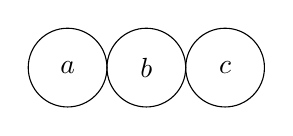
\begin{tikzpicture}
  \draw (0.0,0.0) circle (0.5cm);
  \draw (1.0,0.0) circle (0.5cm);
  \draw (2.0,0.0) circle (0.5cm);
  \node at (0.0,0.0) {$a$};
  \node at (1.0,0.0) {$b$};
  \node at (2.0,0.0) {$c$};
\end{tikzpicture}
\caption{Transitive connection}
\label{wan:fig:cluster}
\end{figure}

The property \cnst{tc} allows us for defining the concept of \textsc{cluster} (\cnst{clstr}) \citep[144]{grimm2012number}. According to \REF{wan:form:cluster}, an entity $x$ is a cluster relative to a connection relation $C$ and a property $P$ iff $x$ is a sum of entities falling under the same property, which are all transitively connected relative to a subset of $Z$ under the same property and connection relation.\footnote{The formula in \REF{wan:form:cluster} also differs from \citeauthor{grimm2012number}'s original definition. The main modification is that I restrict the variable $Y$ to the subsets of $Z$. Without this restriction if, e.g., $P=\{z_1,z_2,z_3\}$, $Z=\{z_1,z_3\}$, $z_1$ and $z_2$ are connected, $z_2$ and $z_3$ are connected and nothing else is connected, then $z_1$ and $z_3$ are transitively connected via $Y=\{z_1,z_2,z_3\}$, which is a subset of $P$, so counterintuitively $z_1 \sqcup z_3$ form a cluster relative to $P$ and $C$ even though it is not a connected entity. Again, I would like to thank Nina Haslinger for pointing this out.} Hence, the sum $a\sqcup b\sqcup c$ in \figref{wan:fig:cluster} is a cluster.

\ea $\cnst{clstr}_{C}(P)(x) \eqdef \exists Z[x = \bigsqcup Z \wedge \forall z \forall z' \in Z \exists Y \subseteq Z[\cnst{tc}(z,z',P,C,Y)]]$\label{wan:form:cluster}
\z

\noindent The notion of \cnst{clstr} as defined in \REF{wan:form:cluster} allows for modelling certain spatial configurations of entities as complex mereotopological objects. In the next section, I will discuss a further extension of the ontology, which will involve roles. 

\section{Roles}\label{wan:sec:roles}

In order to explain the behavior of social collectives, I will follow \citet{zobel2017sensitivity} and extend the usually assumed ontology of the model with an additional domain, namely the domain of \textsc{roles}. Though this is rather uncommon in natural-language semantics (but see \citealt{de-swart_winter_zwarts2007bare} for a related notion of \textsc{capacity}), the relevance of roles as independent ontological objects has been argued for in the literature on theoretical computer science, conceptual modelling and knowledge representation (e.g., \citealt{sowa1984conceptual,steimann2000representation,loebe2007abstract}).

\subsection{Roles vs. individuals}\label{wan:sec:roles-vs-individuals}

On an intuitive level, roles are certain functions or capacities of individuals. As such they are social constructs that are independent of their bearers and there is solid evidence that natural language is sensitive to the distinction between the two. As argued convincingly by \citet{zobel2017sensitivity}, a number of linguistic phenomena demonstrate the relevance of distinguishing between class nouns, i.e., nouns denoting properties of individuals, and role nouns, i.e., nouns denoting properties of roles that individuals can bear.

First of all, certain predicates are sensitive to the distinction in question. For instance, consider the contrast in \REF{wan:ex:judge-man-earn} \citep[see also][]{szabo2003qualification}. Here, \textit{earns 3,000 euros} selects only for as-phrases whose complement is a role noun, thereby \REF{wan:ex:man-earn} is infelicitous. Notice also that \REF{wan:ex:judge-earn} does not convey any information on the total income Paul makes but only on the amount of money he earns for fulfilling this particular role.

		\ea\judgewidth{\#}\label{wan:ex:judge-man-earn} \ea[]{Paul earns 3,000 euros as a judge.}\label{wan:ex:judge-earn}
		\ex[\#]{Paul earns 3,000 euros as a man. \hfill \citep[439]{zobel2017sensitivity}}\label{wan:ex:man-earn}
		\z
        \z

\noindent Moreover, role nouns differ from class nouns with respect to certain entailment patterns, as demonstrated in (\ref{wan:ex:man-hangman-strike}--\ref{wan:ex:judge-hangman-strike}) \citep[see][]{landman1989groupsii}. While the truth of \REF{wan:ex:hangman-strike} is guaranteed by the truth of the premises, the conclusion in \REF{wan:ex:hangman-strike-role} is invalid. 
		
		\ea\judgewidth{$\vDash$}\label{wan:ex:man-hangman-strike} \ea[]{The man (over there) is on strike.}\label{wan:ex:man-strike}
		\ex[]{The man (over there) is the hangman.}\label{wan:ex:man-hangman}
		\ex[$\vDash$]{The hangman is on strike. \hfill \citep[439]{zobel2017sensitivity}}\label{wan:ex:hangman-strike}
		\z
		\ex\label{wan:ex:judge-hangman-strike} \ea[]{The judge is on strike.}\label{wan:ex:judge-strike}
		\ex[]{The judge is the hangman.}\label{wan:ex:judge-hangman}
		\ex[$\nvDash$]{The hangman is on strike. \hfill \citep[724]{landman1989groupsii}}\label{wan:ex:hangman-strike-role}
		\z
		\z

\noindent Another piece of evidence comes from the behavior of the two types of nouns in copular sentences. For instance, German role nouns can appear bare in such environments, see \REF{wan:ex:article-judge}, whereas class nouns cannot, see \REF{wan:ex:article-man}. Similar contrasts are also attested, e.g., in Dutch and French \citep{de-swart_winter_zwarts2007bare}. 

\ea\label{wan:ex:article-judge-man} \ea[]{\gll Paul ist \minsp{(} ein) Richter.\\  
     Paul is {} a judge\\
\glt `Paul is a judge.'}\label{wan:ex:article-judge}
\ex[]{\gll Paul ist \minsp{*(} ein) Mann.\\  
     Paul is {} a man\\ 
\glt `Paul is a man.' \hfill \citep[German;][439, adapted]{zobel2017sensitivity}}\label{wan:ex:article-man}
\z
\z

\noindent A single role can be played by multiple individuals (often at once), see \REF{wan:ex:multiple}, or there can be no individual at all that plays it, see \REF{wan:ex:empty}.\footnote{Naturally, it is also the case that one individual can play multiple roles.}
		
		\ea\label{wan:ex:multiple-empty} \ea[]{The three core players and their organizations are executive director of the Tri-County regional planning commission.}\label{wan:ex:multiple}
		\ex[]{I long for the day when no one is head of the house.  \\ \hfill \citep[449]{zobel2017sensitivity}}\label{wan:ex:empty}
        \z
        \z

\noindent Finally, roles can have properties that do not apply to the individuals fulfilling them. This is witnessed by the use of DPs such as \textit{this role} in argument position, as in \REF{wan:ex:this-role}. It might also be the case that an individual acquires certain properties stemming from duties, obligations and rights associated with playing their role that expire once they stop playing that role, e.g., consider the role of the prime minister or a spouse.

\ea[]{I submit that this role is outmoded and dangerous. \hfill \citep[450]{zobel2017sensitivity}}\label{wan:ex:this-role}
\z

\noindent Now, with the evidence for the relevance of roles for natural language discussed let us review how it can be accounted for formally.

\subsection{Capturing class nouns and role nouns}\label{wan:sec:capturing-class-nouns-and-role-nouns}

I follow \citet{zobel2017sensitivity} in assuming the primitive type $r$ for social roles, which are modeled as independent ontological objects. Hence, alongside the domain of individuals $D_e$ there is also the domain of roles $D_r$. While class nouns denote properties of individuals (type $\stb{e,t}$), see \REF{wan:form:class}, role nouns denote properties of roles (type $\stb{r,t}$), see \REF{wan:form:role}.

\ea \ea \sib{man}${ } = \lambda x_e[\textsc{man}(x)]$\label{wan:form:class}
\ex \sib{judge}${ } = \lambda r_r[\textsc{judge}(r)]$\label{wan:form:role}
\z
\z

\noindent Similarly to individuals, which are referred to by proper names and definite descriptions, particular roles can be designated by dedicated linguistic expressions. Examples include phrases such as the infamous \textit{Grand Wizard} and \textit{President of the United States} as well as demonstrative DPs like \textit{this role} and \textit{that job}.

Importantly, though roles are distinct from individuals, the two ontological categories are closely associated with each other as individuals typically perform roles. This fact is captured by a special shifting operator \cnst{play}, which relates a role with individuals that perform it. As defined in \REF{wan:form:play}, \cnst{play} takes a set of roles $P$ and yields a set of (potentially plural) individuals $x$ for which there are a role $r$ and an eventuality $e$ such that $r$ is a $P$-role and $\langle r,e\rangle$ is part of the specific role structure $\mathscr{R}_x$ of $x$, which structures individuals' participation in eventualities relative to the roles they perform, see \REF{wan:form:role-structure} \citep[451]{zobel2017sensitivity}. 

\ea[]{\sib{\cnst{play}}${ } =\lambda P_{\stb{r,t}} \lambda x_e \exists r_r \exists e_e[P(r) \wedge \langle r,e\rangle \in \mathscr{R}_x]$}\label{wan:form:play}
\ex[]{For each individual $x$, the specific role structure $\mathscr{R}_x$ is a set of role-eventuality-pairs. A pair $\stb{r,e}$ is a member of $\mathscr{R}_x$ iff $x$ is a participant of $e$ in role $r$.}\label{wan:form:role-structure}
\z

\noindent With all the theoretical ingredients in place, let us move on to the proposal.

\section{Collectives as clusters}\label{wan:sec:collectives-as-clusters}

\begin{sloppypar}
In this section, I propose a semantic analysis of Slavic derived collective nouns as properties of clusters. My proposal builds on the mereotopological treatment of aggregate nominals developed by \citet{grimm2012number} and \citet{grimm_docekal-toappear-counting} as well as \citeposst{zobel2017sensitivity} theory of roles. The main claim is that mereotopological relations hold not only between concrete objects occupying physical space but also between abstract entities such as roles in social space. This extension enables us to capture spatial collectives as predicates true of spatial clusters and social collectives as predicates true of social clusters, i.e., pluralities of abstract capacities conceptualized as being socially connected.
\end{sloppypar}

\subsection{Pluralities of roles}\label{wan:sect:pluralities-of-roles}

I propose that not only are roles independent ontological objects, as postulated by \citet{zobel2017sensitivity}, but also that just like ordinary individuals they enter part-whole relations and form pluralities. The evidence comes from the behavior of conjunction within as-phrases. For instance, consider the analogy in \REF{wan:ex:conjunction}.\footnote{I would like to thank Kurt Erbach for his judgments and the discussion of the English examples. The same analogy is also attested in other languages, e.g., German and Polish.} 

\ea\label{wan:ex:conjunction} \ea Paul gave 4,000 euros to Tom and Amy.\label{wan:ex:conjunction-individuals}
\ex Paul earns 4,000 euros as a judge and a lecturer.\label{wan:ex:conjunction-roles}
\z
\z

\noindent The conjoined DP in \REF{wan:ex:conjunction-individuals} gives rise to the well-studied ambiguity between the distributive and the non-distributive construal, i.e., Tom and Amy got either 4,000 euros each or 4,000 euros between them. Likewise, \REF{wan:ex:conjunction-roles} is ambiguous in a very similar way. On the distributive reading, Paul earns 4,000 euros working as a judge and 4,000 euros working as a lecturer, i.e., 8,000 euros in total. In addition, the sentence can be understood in a non-distributive way, i.e., that Paul earns a total of 4,000 euros for both of those two jobs.

Given the evidence described above, it is justified to analyze conjoined role nouns as denoting pluralities of roles built from the denotations of the conjuncts. Such a postulate fits into the general trend in semantic research, which has gradually extended pluralities from the domain of individuals to the domains of events \citep{bach1986algebra}, information states \citep{krifka1996parametrized}, times \citep{arstein_francez2003plural} and degrees \citep{dotlacil_nouwen2016comparative} as well as propositions \citep{lahiri2002questions}, questions \citep{beck_sharvit2002pluralities} and functions \citep{schmitt2019pluralities}.

\subsection{Mereotopology in the social space}\label{wan:sec:mereotopology-in-the-social-space}

It is typically assumed that mereological relations hold not only between concrete physical objects but also between abstract entities. As discussed in the previous section, there are good reasons to maintain that this is also true with respect to roles. On the other hand, in \sectref{wan:sec:mereotopological-structures-in-natural-language} we have seen evidence that the manner in which parts of a whole are arranged with respect to each other is linguistically relevant. The main claim of this paper is that mereotopological relations apply not only in the domain of concrete physical objects but also in the domain of abstract social roles.

In other words, I assume that both individuals and roles are conceptualized as occupying positions within regions of space. The former are located in physical space whereas the latter inhabit abstract \textsc{social space}. At first blush, this idea might seem somewhat controversial but I will argue that the distinction is in fact relevant for natural language. As biological creatures, of course we occupy physical space but as \citet[123]{churchland1996engine} puts it ``we live also in an intricate space of obligations, duties, entitlements, prohibitions, appointments, debts, affections, insults, allies, contracts, enemies, infatuations, compromises, mutual love, legitimate expectations, and collective ideals''. For our species the ``topology'' of this social space is as real and (at least) as important as the topology of the physical space our bodies occupy. Therefore, I believe that it is conceptually plausible that this fact is also reflected in language.

This intuition seems to be supported by the existence of a class of expressions such as \textit{connected}, \textit{close} and \textit{separate} that are systematically polysemous between spatial and social relations. This suggests that the way in which connection is conceptualized in natural language goes beyond spatial connectedness. The notion of social space as part of the semantic model theory would be a way to capture the non-accidental nature of this correspondence.

Hence, I propose to extend mereotopology to abstract domains. The core intuition behind this postulate is that in the case of abstract entities the manner in which their parts are arranged can be as relevant as in the case of concrete individuals. Of course, this move requires abstracting from the connectedness relation \cnst{c} as a relation between physical objects and viewing it as a purely abstract notion that can hold between entities of any type (similarly to the parthood relation $\sqsubseteq$). Here, I will assume two cases of \cnst{c}, specifically \textsc{spatial connection} (\cnst{sp}) and \textsc{social connection} (\cnst{sc}). The former is defined over the domain of individuals in physical space (let us assume here that it simply amounts to $D_e$) whereas the latter is defined over $D_r$, i.e., the domain of roles, which inhabit social space. 

What would it then mean that two roles are connected? One intuitive way of making sense of the concept of social connection is by thinking of shared capacities and obligations that center around a certain well-defined aspect of social life or stem from socially significant relationships between roles \citep[see also][]{joosten2010collective}. This way an institution, i.e., a complex web of model interactions and dependencies, can arise. As a result, individuals performing connected roles are expected to be involved in similar situations and to exhibit a similar type of behavior in role-related events. For instance, roles of family members involve overlapping duties, affections and expectations, and thus can be viewed as connected. Notice, however, that these obligations and relationships should be viewed as regarding primarily roles and not particular individuals. Thus, the reason why it makes sense to talk about peasantry as a social class is not necessarily because individual peasants co-operate with each other but rather because the role of a peasant is defined in terms of a particular type of relationship with the role of a landlord irrespective of who exactly plays that role. 

The extension proposed above allows us to derive more complex mereotopological notions for the domain of roles on a par with what we have already discussed in \sectref{wan:sec:mereotopology}. This in turn enables the modelling of certain pluralities of roles as clusters.

\subsection{Spatial and social clusters}\label{wan:sec:spatial-and-social-clusters}

I propose that both spatial and social collectives in Slavic denote properties of clusters. Hence, on a general level they are closely related expressions. However, the crucial difference between the two concerns the kind of entities that form a cluster and, consequently, the kind of connection relation holding between them.

Based on the generalization in \REF{wan:ex:generalization}, I argue that all Slavic collective suffixes form a natural class consisting of the spatial and the social subtype. Since spatial collectives demonstrably make reference to clusters and the derivational processes yielding these expressions belong to a larger class that should receive a unified semantics, I postulate that all derivational suffixes for collective nouns involve the notion of a cluster in some way. Together with the independently motivated idea that social collectives denote predicates of pluralities of roles, this entails that they involve clusters in social space. In \REF{wan:form:coll}, I propose a schematic lexical entry for Slavic collective suffixes (\textsc{-coll}) that specifies every aspect of their meaning except the type of the noun they are suffixed to. Specifically, \mbox{\textsc{-coll}} takes a predicate of type $\stb{\alpha,t}$, where $\alpha$ ranges over primitive types ($e$ and $r$ in particular), and yields a set of clusters relative to the relevant property and connection relation. In other words, the result is a semantically plural expression denoting predicates true of cluster individuals of type $e$ or $r$.

\ea \sib{\textsc{-coll}}${ } =\lambda P_{\stb{\alpha,t}} \lambda x_\alpha[\cnst{clstr}_{\cnst{c}}(P)(x)]$\label{wan:form:coll}
\z

\noindent Following the analysis of Czech derived aggregate nouns by \citet{grimm_docekal-toappear-counting}, I posit that Slavic derived spatial collectives refer to clusters of objects in physical space. The denotation of the Polish suffix \textit{-e} is given in \REF{wan:form:e}, where \cnst{sp} stands for a spatial connection between physical entities.\footnote{\REF{wan:form:e} differs from \citeauthor{grimm_docekal-toappear-counting}'s proposal with the main difference being that they are also interested in the relationship between objects and kinds, which I ignore here.} Thus, \textit{-e} takes a property of individuals and yields a set of spatial clusters. For instance, when it attaches to \REF{wan:form:kwiat}, what we obtain is a set of clumps of flowers, see \REF{wan:form:spatial-cluster}.

\ea \ea \sib{-e}${ } =\lambda P_{\stb{e,t}} \lambda x_e[\cnst{clstr}_{\cnst{sp}}(P)(x)]$\label{wan:form:e}
\ex \sib{kwiat}${ } =\lambda x_e[\textsc{flower}(x)]$\label{wan:form:kwiat}
\ex \sib{kwiecie}${ } =\lambda x_e[\cnst{clstr}_{\cnst{sp}}(\textsc{flower})(x)]$\label{wan:form:spatial-cluster}
\z
\z

\noindent Let us now demonstrate linguistic evidence that social collectives do in fact involve reference to roles. First, \REF{wan:ex:money} has a reading on which it can be true even if individual members of the clergy received money from the state, as long as these subsidies were unrelated to their role as clergy.

\ea[]{\gll Duchowieństwo nie otrzymało żadnych pieniędzy od państwa.\\
priest\textsc{.coll} \textsc{neg} received any\textsc{.gen} money\textsc{.gen} form state\textsc{.gen}\\
\glt `The clergy did not receive any money from the state.' \hfill (Polish)}\label{wan:ex:money}
\z

\noindent Furthermore, arguments such as \REF{wan:ex:delegation-clergy-strike} have a reading on which they are invalid, similarly to \REF{wan:ex:judge-hangman-strike}. For instance, the conclusion in \REF{wan:ex:delegation-strike} does not necessarily follow from the premises in \REF{wan:ex:delegation-clergy} and \REF{wan:ex:clergy-strike} if the delegation is intended to represent interests of the local community rather than the official position of the church.

\ea\judgewidth{$\nvDash$}\label{wan:ex:delegation-clergy-strike}
\ea[]{\gll Delegacja na szczyt klimatyczny składa się z lokalnego duchowieństwa.\\
delegation on summit\textsc{.acc} climate\textsc{.adj} consists \textsc{refl} from local\textsc{.gen} priest\textsc{.coll.gen}\\
\glt `The delegation to the climate summit consists of the local clergy.'}\label{wan:ex:delegation-clergy}
\ex[]{\gll Lokalne duchowieństwo strajkuje.\\
local priest\textsc{.coll} is.on.strike\\
\glt `The local clergy are on strike.'}\label{wan:ex:clergy-strike}
\ex[$\nvDash$]{\gll Delegacja na szczyt klimatyczny strajkuje.\\
delegation on summit\textsc{.acc} climate\textsc{.adj} is.on.strike\\
\glt `The delegation to the climate summit is on strike.' \hfill (Polish)}\label{wan:ex:delegation-strike}
\z
\z

\noindent With this in mind, let me now propose a semantics for derived social collectives. As already mentioned, the core idea is that they are essentially very similar to spatial collective nouns, with the crucial difference that the \cnst{clstr} operation is now relativized to \cnst{sc}, and thus applies to roles. As evident in the formula in \REF{wan:form:stwo}, the Polish suffix \textit{-stwo} selects a property of roles and returns a set of clusters of roles formed relative to that property. For instance, when \textit{-stwo} combines with \REF{wan:form:duchowny}, the result in \REF{wan:form:social-cluster} is a predicate true of clusters of priest roles corresponding to a clerical organization. If needed, this predicate can be associated with particular individuals performing those roles via the shifting operator \cnst{play}. As a result, we can account for the dual life of social collectives, i.e., the fact that they designate an abstract social entity that can have different properties than its constituent members, but at the same time we can talk about the constituent members using a collective noun.  

\ea \ea \sib{-stwo}${ } =\lambda P_{\stb{r,t}} \lambda r_r[\cnst{clstr}_{\cnst{sc}}(P)(r)]$\label{wan:form:stwo}
\ex \sib{duchowny}${ } =\lambda r_r[\textsc{priest}(r)]$\label{wan:form:duchowny}
\ex \sib{duchowieństwo}${ } =\lambda r_r[\cnst{clstr}_{\cnst{sc}}(\textsc{priest})(r)]$\label{wan:form:social-cluster}
\z
\z

\noindent The proposed analysis has two important advantages. First of all, it captures the intuition that the two types of collective nouns are actually closely related since they both make use of the \cnst{clstr} operator. At the same time, it also explains the source of the differences between spatial and social collectives, as examined in \sectref{wan:sec:types-of-collectives} and \sectref{wan:sec:slavic-derived-collectives}. Specifically, the \cnst{clstr} operator accounts for collective inferences whereas different types of connection, i.e., \cnst{sp} and \cnst{sc}, correspond to the two distinct modes of collectivity discussed in \sectref{wan:sec:modes-of-collectivity}.

The proposal captures the core properties of spatial and social collections in the following manner. The reason why spatial collections may cease to exist when the topological configuration of their constituent members is rearranged, as in \REF{wan:ex:entailment-committee}, is simply because the spatial connection relative to which the cluster is defined does not apply anymore, and thus there is no cluster anymore. On the other hand, the location of individuals who perform roles making up a social cluster is irrelevant, recall (\ref{wan:ex:entailment-bouquet}--\ref{wan:ex:entailment-fleet}), because the cluster is not defined in spatial space, but rather in the abstract social space. In relation to this, the fact that social collections appear to exist independently of their constituent members, recall \REF{wan:ex:no}, stems straightforwardly from the different ontological status of social clusters (type $r$) as compared to individuals (type $e$). Consequently, there can be very few or even no individuals performing the relevant roles at a given moment, which also accounts for the contrast in (\ref{wan:ex:plurality}--\ref{wan:ex:plurality-fleet}). Finally, the compatibility of certain predicates, e.g., the Polish verb \textit{należeć} `belong', only with social collectives, recall \REF{wan:ex:belong}, can be easily explained by postulating a selectional restriction requiring an expression of type $\stb{r,t}$.

\section{Conclusion}\label{wan:sec:conclusion}

In this paper, I have discussed data showing that Slavic morphology reflects two different modes of collectivity. In particular, I have examined two types of derived collective nouns, i.e., spatial collectives such as Polish \textit{kwiecie} `clump of flowers' and social collectives like \textit{duchowieństwo} `collective of priests, clergy'. Building on a mereotopological approach to nominal semantics \citep{grimm2012number} and theory of roles \citep{zobel2017sensitivity}, I have argued that the former denote properties of spatial clusters, i.e., topologically structured aggregates of entities in physical space, whereas the latter designate properties of social clusters, i.e., abstract configurations of social roles individuals can perform that constitute institutions. Therefore, both spatial and social collectives make reference to the same type of complex mereotopological structure, the only difference being whether it is defined in the domain of individuals or in the domain of roles. The findings provide novel evidence for a more fine-grained typology of collectives and a richer natural-language ontology.

\section*{Abbreviations}


\begin{tabularx}{.5\textwidth}{@{}lX@{}}
\textsc{acc}&{accusative}\\
\textsc{adj}&{adjective}\\
\textsc{coll}&{collective}\\
\end{tabularx}%
\begin{tabularx}{.5\textwidth}{@{}lX@{}}
\textsc{gen}&{genitive}\\
\textsc{neg}&{negation}\\
\textsc{refl}&{reflexive}\\
\end{tabularx}

\section*{Acknowledgements}

I would like to sincerely thank two anonymous reviewers for their helpful comments and questions. Furthermore, I am especially grateful to Nina Haslinger, Hanna de Vries, Sarah Zobel and Joost Zwarts for inspiring discussions about collectivity, mereotopology and roles as well as the following persons for the discussion of the data: Boban Arsenijević (BCMS), Kurt Erbach (American English), Izabela Jordanoska (Macedonian), Petra Mišmaš (Slovenian), Mariia Onoeva (Russian), Peter Sutton (British English), and Lucia Vlášková (Slovak). All errors are, of course, my own responsibility. I gratefully acknowledge that the research was supported by a Czech Science Foundation (GAČR) grant to the Department of Linguistics and Baltic Languages at the Masaryk University in Brno (GA20-16107S).

{\sloppy\printbibliography[heading=subbibliography,notkeyword=this]}

\end{document}
